\section{MARCO TEORICO} 
		
\begin{enumerate}[1.]
	\item Business Analytics :
\\
\\
Al igual que la inteligencia de negocios, BA recopila y analiza datos, emplea análisis predictivos y genera informes visualizados en paneles personalizados. El objetivo de estas características es ayudar a identificar y abordar los puntos débiles de una organización. Aquí es donde terminan las similitudes. El software de análisis de negocios se utiliza para explorar y analizar datos históricos y actuales. Utiliza el análisis estadístico, la extracción de datos y el análisis cuantitativo para identificar las tendencias comerciales anteriores.
\\
Una vez que se han recopilado y analizado los datos, los sistemas de análisis de inteligencia empresarial los utilizan para el modelado predictivo. Esto puede predecir y, en la mayoría de los casos, prepararse para futuros climas empresariales. Uno de los aspectos más poderosos de BA es el informe ad-hoc, que permite a las empresas realizar análisis de datos específicos en tiempo real para responder preguntas específicas para tomar decisiones comerciales más rápidas. En efecto, el análisis de negocios utiliza el análisis predictivo para resolver problemas antes de que hayan ocurrido.

\end{enumerate}

\begin{center}
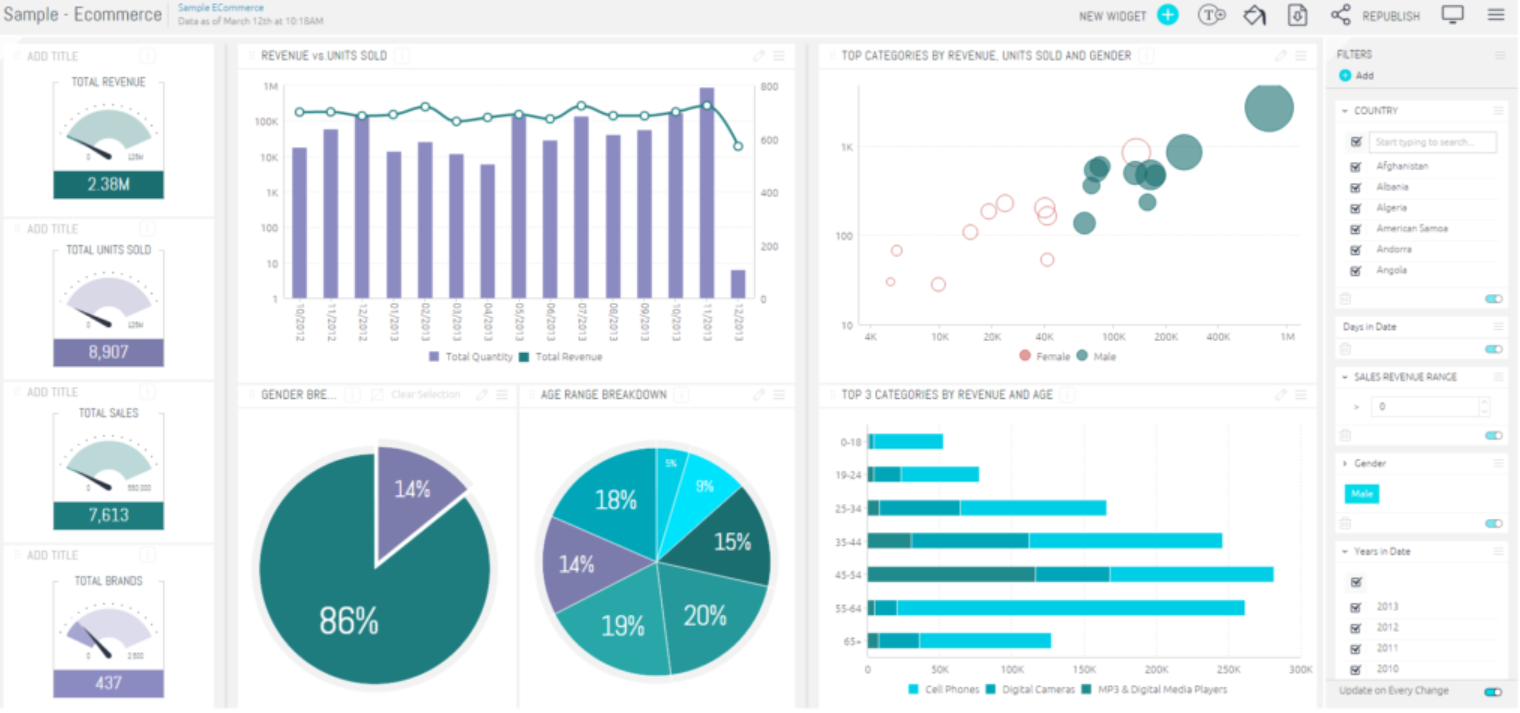
\includegraphics[scale=0.55]{./Imagenes/BA.png}
\end{center}

\begin{enumerate}[2.]
	\item Business Intelligence:
\\
\\
La inteligencia de negocios o business intelligence (BI) es el conjunto de procesos, aplicaciones y tecnologías que facilitan la obtención rápida y sencilla de datos provenientes de los sistemas de gestión empresarial para su análisis e interpretación, de manera que puedan ser aprovechados para la toma de decisiones y se conviertan en conocimiento para los responsables del negocio.
Esta tecnología actúa como un factor clave y estratégico para la organización ya que provee a los tomadores de decisiones de información oportuna y confiable para responder a las situaciones que puedan presentarse en la empresa como son la entrada a nuevos mercados, el análisis de costos, la rentabilidad de una línea de productos, etc.

La información brindada por el BI puede tener distintos alcances como son:
\\
\\\\- Brindar al estudiante los conocimientos necesarios para realizar la Instalación de un servidor de Base de Datos Oracle sobre el sistema operativo Windows Server 2012 R2.
	\\- Nivel operativo: En este rubro es utilizado para la toma de decisiones diarias acerca de las transacciones que se realizan al llevar a cabo las operaciones de la empresa.\\
	\\- Nivel tactica: aporta informacion para los mandos medios en analisis y decisiones mensuales que son de utilidad para revisiones de seguimiento y toma de acciones.\\
	\\- Nivel estrategico: A este nivel las decisiones son de mayor impacto en la compañia siendo utilizada la informacion por a alta direccion.\\


Las herramientas de inteligencia de negocios por lo general muestran la información en forma de cuadros de mando o  tableros de control y los informes específicos que se pueden crear a partir de los datos que se obtienen de ERP que la empresa utiliza para su gestión, de tal forma que La información se presenta al usuario de manera ágil y accesible para que pueda utilizar el análisis e interpretación correspondiente.

La información brindada por el BI puede tener distintos alcances como son:\\
\\- Mercadotecnia: en esta area el BI puede ser aprovechado para segmentacion de mercados, analisis de tendencias y de clientes.\\
\\- Ventas: analisis de clientes y su rentabilidad, analisis por producto, por segmento, proyecciones y pronosticos de ventas.\\
\\- Finanzas: reportes detallados de gastos, costos e ingresos asi como para razones financieras y analisis financiero de la empresa.\\
\\- Logistica: seguimiento de embarques y monitoreo de pedidos para saber la causa de su perdida.\\
\\- Produccion: reporte de productividad de lineas de produccion, rotacion de inventarios, etc.\\




\end{enumerate}

\begin{center}
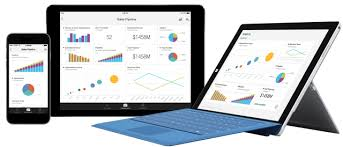
\includegraphics[scale=0.90]{./Imagenes/1.png}
\end{center}

Algunas de las ventajas que puedes tener en tu empresa al utilizar la inteligencia de negocios son las siguientes: 

-Incremento de la eficiencia: Al contar con los datos de manera accesible y ágil puedes generar información de valor centralizada la cual podrás visualizar en una única plataforma para aprovecharla de manera óptima para realizar análisis y tomar decisiones informadas y en tiempo.\\

-Respuestas rápidas a situaciones de negocio: Para poder tomar decisiones en el momento indicado es importante contar con la información a la mano de manera sencilla y no perder tiempo en buscar y consolidar datos. Gracias al BI puedes tener las respuestas en minutos de manera clara y concisa por medio de reportes de indicadores y tableros de datos.\\

-Control de las áreas funcionales de la empresa: En todas las áreas de tu empresa se genera información de valor día a día, puedes aprovecharla de la mejor manera para conocer tendencias, proyectar datos, analizar escenarios, etc.\\

-Mejora tu servicio al cliente: Al contar con la información más importante y en tiempo real puedes ofrecer a tus clientes un servicio de mayor calidad desde el pedido hasta el servicio post-venta al conocer más acerca de ellos y sus necesidades. Analiza hábitos de compra, reconoce los productos más vendidos, etc.\\

-Presenta información por medio de tableros de indicadores para una comunicación más simple y directa de la situación de la empresa. Al tener la posibilidad de crear distintos tableros para control puedes enfocarte en los datos más relevantes que mostrar sin necesidad de revisar grandes cantidades de información.\\


\begin{enumerate}[3.]
	\item Diferencia entre Business Analytics (BA) y Business Intelligence (BI) :
\\
\\
La diferencia radica en que BA hace un uso extensivo de los datos, análisis estadístico, modelos explicativos y predictivos para empujar la toma de decisiones. Por otro lado, BI está más unida a la creación de los datos e información para apoyar el mismo proceso. Hay dos factores importantes que se tienen diferenciar:
\\
\\
Una vez que se han recopilado y analizado los datos, los sistemas de análisis de inteligencia empresarial los utilizan para el modelado predictivo. Esto puede predecir y, en la mayoría de los casos, prepararse para futuros climas empresariales. Uno de los aspectos más poderosos de BA es el informe ad-hoc, que permite a las empresas realizar análisis de datos específicos en tiempo real para responder preguntas específicas para tomar decisiones comerciales más rápidas. En efecto, el análisis de negocios utiliza el análisis predictivo para resolver problemas antes de que hayan ocurrido.
\\
\\
	- El aspecto comercial de BI, es decir, la necesidad de obtener el máximo valor de la información. Esta necesidad no ha cambiado en más de cincuenta años (a pesar de la creciente complejidad de la economía mundial). La mayoría de los verdaderos problemas que nos impiden obtener el valor de la información (cultura de la información, la política, la falta de competencia analítica, etc.) tampoco han cambiado mucho en las últimas décadas.
\\
\\
	- El aspecto tecnológico de BI, es decir, lo que la tecnología utiliza para ayudar a satisfacer las necesidades del negocio. Los problemas de nomenclatura normalmente surgen porque “inteligencia de negocios” es comúnmente utilizado para referirse a la parte tecnológica, confundiendo así a todo el mundo.
\\
\\
El BA usa una serie de técnicas del tradicional BI, pero el BA es un mix de análisis de escenarios y minería de datos. El BA es una tendencia, un pedido de los usuarios que buscan la diferenciación. Business Intelligence se necesita para manejar un negocio, mientras Business Analytics se necesita para cambiar un negocio.
\\
\\
Business analytics depende un volumen suficiente de datos de alta calidad. La dificultad en asegurar datos de calidad está en integrar y recolectar datos de los diferentes sistemas y luego decidir qué tipo de data poner a disposición.
\\
\\
Previamente BA era considerado un tipo de método “después del hecho” del comportamiento del consumidor examinando el número de unidades vendidas en el último trimestre del periodo. Este tipo de data requiere mucho espacio de almacenamiento que velocidad. Hoy en día BA se está convirtiendo en una herramienta que puede influenciar el resultado de la interacción de los consumidores. Cuando un cliente específico es considerado una compra, una empresa que aplica analytics puede modificar el argumento de venta para atraer ese consumidor. Esto quiere decir que la capacidad de memoria de data puede reaccionar extremadamente rápido para proveer la información necesaria en tiempo real.
\\
\\
El Business Analytics ofrece ventaja competitiva tanto a empresas grandes como pequeñas. En situaciones donde existe gran cantidad de datos, puede ser muy útil. El análisis avanzado puede facilitar una manera práctica de recopilar, limpiar, relacionar y analizar los datos esos.
\\
\\
La disponibilidad de grandes cantidades de datos ha creado en las empresas la necesidad de contar con profesionales que puedan analizar estos datos y obtener el conocimiento necesario para la tomar decisiones informadas. Esto permite que una organización obtenga ventaja competitiva en el entorno empresarial tan dinámico de hoy.
\\
\\
BA usa los datos empresariales para favorecer a otras empresas a tomar decisiones fundamentales para su negocio. Almacenar datos de internet y de las redes sociales corporativas le da a la empresa una fuente de información que le será muy útil para su actividad. Entonces podemos respaldar el hecho de que los datos online forman parte de BA. Es tal la contribución de las actividades online de una las empresas, que muchas han integrado sus datos online en un sistema de información y procesos de toma de decisiones.
\\
\\
Thomas Davenport, profesor de tecnología y gestión de la información en Babson College argumenta que las empresas pueden optimizar una capacidad de negocio distinta a través de analytics para así competir mejor. Él identifica estas características de una organización que es apta para competir en analytics:

	- Uno o más altos ejecutivos que defienden firmemente la toma de decisiones basada en hechos y, en concreto, de análisis.
\\
\\
	- El uso generalizado no sólo de la estadística descriptiva , sino también modelos de predicción y técnicas de optimización complejos
\\
\\
	- El uso sustancial de la analítica a través de múltiples funciones o procesos de negocio.
\\
\\
	- El movimiento hacia un enfoque a nivel de empresa para la gestión de herramientas de análisis, los datos y las habilidades y capacidades de la organización.



\end{enumerate}

\begin{center}

\includegraphics[scale=0.55]{./Imagenes/ba2.jpg}
\end{center}


